\subsection{Enumeration field values}
\label{subsec:library_of_transformations:instance_level_transformations:enum_field_values}

\begin{figure}
    \centering
    \begin{subfigure}{0.95\textwidth}
        \centering
        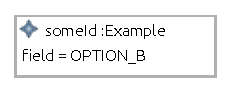
\includegraphics{images/05_library_of_transformations/03_instance_level_transformations/07_enum_field_values/enum_field_value.pdf}
        \caption{$Im_{EnumField}$ with one object and its field referencing enumeration option $OPTION\!\_B$}
        \label{fig:library_of_transformations:instance_level_transformations:enum_field_values:visualisation:ecore}
    \end{subfigure}
    \\
    \begin{subfigure}{0.95\textwidth}
        \centering
        % To use this figure in your LaTeX document
% import the package groove/resources/groove2tikz.sty
%
\begin{tikzpicture}[scale=\tikzscale,name prefix=start-]
\node[basic_node] (n0) at (1.975, -0.185) {\ml{\uline{\textit{someId}} : \textbf{Example}}};
\node[basic_node] (n1) at (5.650, -0.370) {\ml{\uline{\textit{ExistingEnumOptionA}} : \textbf{ExistingEnum\$OPTION\_A}}};
\node[basic_node] (n2) at (1.940, -1.145) {\ml{\uline{\textit{ExistingEnumOptionB}} : \textbf{ExistingEnum\$OPTION\_B}}};
\node[basic_node] (n3) at (5.650, -0.905) {\ml{\uline{\textit{ExistingEnumOptionC}} : \textbf{ExistingEnum\$OPTION\_C}}};

\path[basic_edge](n0.south -| 1.940, -1.145) -- node[lab] {\ml{field}} (n2) ;
\end{tikzpicture}

        \caption{$IG_{EnumFieldNodes}$ with one node and and its edge referencing enumeration option $OPTION\!\_B$}
        \label{fig:library_of_transformations:instance_level_transformations:enum_field_values:visualisation:groove_nodes}
    \end{subfigure}
    \\
    \begin{subfigure}{0.95\textwidth}
        \centering
        % To use this figure in your LaTeX document
% import the package groove/resources/groove2tikz.sty
%
\begin{tikzpicture}[scale=\tikzscale,name prefix=start-]
\node[basic_node] (n0) at (1.975, -0.185) {\ml{\uline{\textit{someId}} : \textbf{Example}}};
\node[basic_node] (n1) at (5.650, -0.370) {\ml{\uline{\textit{ExistingEnumOptionA}} : \textbf{ExistingEnum}\\\textit{OPTION\_A}}};
\node[basic_node] (n2) at (1.940, -1.125) {\ml{\uline{\textit{ExistingEnumOptionB}} : \textbf{ExistingEnum}\\\textit{OPTION\_B}}};
\node[basic_node] (n3) at (5.650, -0.905) {\ml{\uline{\textit{ExistingEnumOptionC}} : \textbf{ExistingEnum}\\\textit{OPTION\_C}}};

\path[basic_edge](n0.south -| 1.940, -1.125) -- node[lab] {\ml{field}} (n2) ;
\end{tikzpicture}

        \caption{$IG_{EnumFieldFlags}$ with one node and its edge referencing enumeration option $OPTION\!\_B$}
        \label{fig:library_of_transformations:instance_level_transformations:enum_field_values:visualisation:groove_flags}
    \end{subfigure}
    \caption{Visualisation of the transformation of field values from fields typed by enumeration types}
    \label{fig:library_of_transformations:instance_level_transformations:enum_field_values:visualisation}
\end{figure}

In this section, the instance level transformation belonging to the transformation of an enumeration field is discussed. The type level transformation for enumeration fields can be found in \cref{subsec:library_of_transformations:type_level_transformations:enum_fields}. On the instance level, values for the enumeration fields are introduced.

\begin{defin}[Instance model $Im_{EnumField}$]
\label{defin:library_of_transformations:instance_level_transformations:enum_field_values:imod_enum_field}
Let $Im_{EnumField}$ be an instance model typed by $Tm_{EnumField}$ (\cref{defin:library_of_transformations:type_level_transformations:enum_fields:tmod_enum_field}). Define a set $objects$, which represent the objects that will get a value for the field introduced by $Tm_{EnumField}$. Furthermore, define a function $obids$ which maps each of these objects to their corresponding identifier and a function $values$, which maps each of these objects to its value for the field introduced by $Tm_{EnumField}$. $Im_{EnumField}$ is defined as:
\begin{align*}
Object =\ &objects \\
\mathrm{ObjectClass} =\ & \begin{cases}
    (ob, classtype) & \mathrm{if }\ ob \in objects
\end{cases}\\
\mathrm{ObjectId} =\ & \begin{cases}
    (ob, obids(ob)) & \mathrm{if }\ ob \in objects
\end{cases}\\
\mathrm{FieldValue} =\ & \begin{cases}
    \Big((ob, (classtype, name)), \big[\type{enum}, (enumid, values(ob))\big]\Big) & \mathrm{if }\ ob \in objects
\end{cases} \\
\mathrm{DefaultValue} =\ & \{\}
\end{align*}
\isabellelref{imod_enum_field}{Ecore-GROOVE-Mapping-Library.EnumFieldValue}
\end{defin}

\begin{thm}[Correctness of $Im_{EnumField}$]
\label{defin:library_of_transformations:instance_level_transformations:enum_field_values:imod_enum_field_correct}
$Im_{EnumField}$ (\cref{defin:library_of_transformations:instance_level_transformations:enum_field_values:imod_enum_field}) is a valid instance model in the sense of \cref{defin:formalisations:ecore_formalisation:instance_models:model_validity}.
\isabellelref{imod_enum_field_correct}{Ecore-GROOVE-Mapping-Library.EnumFieldValue}
\end{thm}

A visual representation of $Im_{EnumField}$ with $objects = \{ob\}$ and $obids(ob) = someId$ can be seen in \cref{fig:library_of_transformations:instance_level_transformations:enum_field_values:visualisation:ecore}. In this visualisation, the field value for $ob$ is defined as $values(ob) = OPTION\!\_B$. Although this visualisation only shows one object, it is required to define a value for all objects that contain the field. Failing to do so would result in an invalid instance model after it is combined with another model, as the next definition will show. The correctness proof of $Im_{EnumField}$ only is quite involved, but not be included here for conciseness. It can be found as part of the validated Isabelle proofs.

In order to make composing transformation functions possible, $Im_{EnumField}$ should be compatible with the instance model it is combined with.

\begin{thm}[Correctness of $\mathrm{combine}(Im, Im_{EnumField})$]
\label{defin:library_of_transformations:instance_level_transformations:enum_field_values:imod_enum_field_combine_correct}
Assume an instance model $Im$ that is valid in the sense of \cref{defin:formalisations:ecore_formalisation:instance_models:model_validity}. Then $Im$ is compatible with $Im_{EnumField}$ (in the sense of \cref{defin:transformation_framework:instance_models_and_instance_graphs:combining_instance_models:compatibility}) if:
\begin{itemize}
    \item All requirements of \cref{defin:library_of_transformations:type_level_transformations:enum_fields:tmod_enum_field_combine_correct} are met, to ensure the combination of the corresponding type models is valid;
    \item The class type on which the field is defined by $Tm_{EnumField}$ may not be extended by another class type in the type model corresponding to $Im$;
    \item All of the objects in the set $objects$ must already be objects in $Im$;
    \item All objects typed by the class type on which the field is defined must occur in the set $objects$ and thus have a value in $Im_{EnumField}$;
    \item For all of the objects in the set $objects$, the identifier set by $obids$ must be the same identifier as set by $Im$ for that object;
    \item For all objects in set $objects$, the value set by the $values$ function must be valid.
\end{itemize}
\isabellelref{imod_enum_field_combine_correct}{Ecore-GROOVE-Mapping-Library.EnumFieldValue}
\end{thm}

\begin{proof}
Use \cref{defin:transformation_framework:instance_models_and_instance_graphs:combining_instance_models:imod_combine_merge_correct}. It is possible to show that all assumptions hold. Now we have shown that $\mathrm{combine}(Im, Im_{EnumField})$ is consistent in the sense of \cref{defin:formalisations:ecore_formalisation:instance_models:model_validity}.
\end{proof}

As explained earlier, $Im_{EnumField}$ needs to introduce values for all objects that are typed by the class type on which the field is defined. This is enforced by the requirements of \cref{defin:library_of_transformations:instance_level_transformations:enum_field_values:imod_enum_field_combine_correct}. The proof is not included here for conciseness, but can be found as part of the validated proofs in Isabelle.

The definitions and theorems for introducing values for fields of data types within Ecore are now complete. 

\subsubsection{Encoding as edges and nodes with a node type encoded enumeration type}

As discussed in \cref{subsec:library_of_transformations:type_level_transformations:enum_fields}, there are two different encodings for a field typed by an enumeration type. These correspond to the two different encodings of the enumeration type itself. On the instance level, these encodings also need to be distinguished. The first encoding of the values assumes that the enumeration is encoded using node types. The encoding corresponding to $Im_{EnumField}$ is then represented as $IG_{EnumFieldNodes}$, defined in the following definition:

\begin{defin}[Instance graph $IG_{EnumFieldNodes}$]
\label{defin:library_of_transformations:instance_level_transformations:enum_field_values:ig_enum_as_node_types_field_as_edge_type}
Let $IG_{EnumFieldNodes}$ be the instance graph typed by type graph $TG_{EnumFieldNodes}$ (\cref{defin:library_of_transformations:type_level_transformations:enum_fields:tg_enum_as_node_types_field_as_edge_type}). Reuse the set $objects$ from $Im_{EnumField}$. Moreover, reuse the functions $obids$ and $values$ from $Im_{EnumField}$. Furthermore, define $enumob$ to be the function that maps an enumeration value to an internal node identity. Similarly, define $enumids$ as the function that maps an enumeration value to its explicit node id.

Within $IG_{EnumFieldNodes}$, the objects in the set $objects$ are converted to nodes in $Im_{EnumField}$. For each of these objects, an edge of the encoded field is created. This edge targets a node that corresponds to the value set by $values$ for the corresponding object. Furthermore, the identity of the objects is defined using $obids$. Finally, ensure that the instances of the enumeration values exist and encode them in the same way as $IG_{EnumNodes}$ (\cref{defin:library_of_transformations:instance_level_transformations:enumeration_values:ig_enum_as_node_types}). $IG_{EnumFieldNodes}$ is defined as:
\begin{align*}
N =\ & objects \cup \{enumob(v) \mid v \in enumvalues \} \\
E =\ & \big\{\big(ob, (\mathrm{ns\_\!to\_\!list}(classtype), \langle name \rangle, \mathrm{ns\_\!to\_\!list}(enumid)), enumob(values(ob))\big) \mid ob \in objects \big\} \\
\mathrm{ident} =\ & \begin{cases}
    (obids(ob), ob) & \mathrm{if }\ ob \in objects\\
    (enumids(v), enumob(v)) & \mathrm{if }\ v \in enumvalues
\end{cases}
\end{align*}
with
\begin{align*}
\mathrm{type}_n =\ & \begin{cases}
    (ob, \mathrm{ns\_\!to\_\!list}(classtype)) & \mathrm{if }\ ob \in objects\\
    (enumob(v), \mathrm{ns\_\!to\_\!list}(enumid) \append \langle v \rangle) & \mathrm{if }\ v \in enumvalues
\end{cases}
\end{align*}
\isabellelref{ig_enum_as_node_types_field_as_edge_type}{Ecore-GROOVE-Mapping-Library.EnumFieldValue}
\end{defin}

\begin{thm}[Correctness of $IG_{EnumFieldNodes}$]
\label{defin:library_of_transformations:instance_level_transformations:enum_field_values:ig_enum_as_node_types_field_as_edge_type_correct}
$IG_{EnumFieldNodes}$ (\cref{defin:library_of_transformations:instance_level_transformations:enum_field_values:ig_enum_as_node_types_field_as_edge_type}) is a valid instance graph in the sense of \cref{defin:formalisations:groove_formalisation:instance_graphs:instance_graph_validity}.
\isabellelref{ig_enum_as_node_types_field_as_edge_type_correct}{Ecore-GROOVE-Mapping-Library.EnumFieldValue}
\end{thm}

A visual representation of $IG_{EnumFieldNodes}$ with $objects = \{ob\}$ and $obids(ob) = someId$ can be seen in \cref{fig:library_of_transformations:instance_level_transformations:enum_field_values:visualisation:groove_nodes}. Like the previous visualisation, the field value for $ob$ is defined as $values(ob) = OPTION\!\_B$. Although this visualisation only shows one node, it is required to define a value for all nodes that are typed by the node type corresponding to the field. Failing to do so would result in an invalid instance graph after it is combined with another graph, as the next definition will show. The correctness proof of $IG_{EnumFieldNodes}$ only is quite involved, but not be included here for conciseness. It can be found as part of the validated Isabelle proofs.

In order to make composing transformation functions possible, $IG_{EnumFieldNodes}$ should be compatible with the instance graph it is combined with.

\begin{thm}[Correctness of $\mathrm{combine}(IG, IG_{EnumFieldNodes})$]
\label{defin:library_of_transformations:instance_level_transformations:enum_field_values:ig_enum_as_node_types_field_as_edge_type_combine_correct}
Assume an instance graph $IG$ that is valid in the sense of \cref{defin:formalisations:groove_formalisation:instance_graphs:instance_graph_validity}. Then $IG$ is compatible with $IG_{EnumFieldNodes}$ (in the sense of \cref{defin:transformation_framework:instance_models_and_instance_graphs:combining_instance_graphs:compatibility}) if:
\begin{itemize}
    \item All requirements of \cref{defin:library_of_transformations:type_level_transformations:enum_fields:tg_enum_as_node_types_field_as_edge_type_combine_correct} are met, to ensure the combination of the corresponding type graphs is valid;
    \item The node type on which the corresponding field is defined is not extended by other node types within the type graph corresponding to $IG$;
    \item All nodes in $IG$ that are typed by the node type on which the field is defined are also nodes in $IG_{EnumFieldNodes}$;
    \item All nodes in $IG_{EnumFieldNodes}$ that encode the values of the corresponding enumeration type are also nodes in $IG$;
    \item For all nodes shared between $IG$ and $IG_{EnumFieldNodes}$, each node must have the same identifier in both $IG$ and $IG_{EnumFieldNodes}$;
    \item For all nodes for which the field is set, the $values$ function must define a valid value.
\end{itemize}
\isabellelref{ig_enum_as_node_types_field_as_edge_type_combine_correct}{Ecore-GROOVE-Mapping-Library.EnumFieldValue}
\end{thm}

\begin{proof}
Use \cref{defin:transformation_framework:instance_models_and_instance_graphs:combining_instance_graphs:ig_combine_merge_correct}. It is possible to show that all assumptions hold. Now we have shown that $\mathrm{combine}(IG, IG_{EnumFieldNodes})$ is valid in the sense of \cref{defin:formalisations:groove_formalisation:instance_graphs:instance_graph_validity}.
\end{proof}

Like the definition for the combination of instance models, the combination of instance graphs also requires the user to set a value for all nodes that are typed by the node type that corresponds to the field type. This is to keep the graph valid.

The next definitions define the transformation function from $Im_{EnumField}$ to $IG_{EnumFieldNodes}$:

\begin{defin}[Transformation function $f_{EnumFieldNodes}$]
\label{defin:library_of_transformations:instance_level_transformations:enum_field_values:imod_enum_field_to_ig_enum_as_node_types_field_as_edge_type}
The transformation function $f_{EnumFieldNodes}(Im)$ is defined as:
\begin{align*}
N =\ & Object_{Im} \cup \{enumob(ob) \mid v \in enumvalues\}  \\
E =\ & \big\{\big(ob, (\mathrm{ns\_\!to\_\!list}(classtype), \langle name \rangle, \mathrm{ns\_\!to\_\!list}(enumid)), enumob(values(ob))\big) \mid \\&ob \in Object_{Im} \big\} \\
\mathrm{ident} =\ & \begin{cases}
    (obids(ob), ob) & \mathrm{if }\ ob \in Object_{Im}\\
    (enumids(v), enumob(v)) & \mathrm{if }\ v \in enumvalues
\end{cases}
\end{align*}
with
\begin{align*}
\mathrm{type}_n =\ & \begin{cases}
    (ob, \mathrm{ns\_\!to\_\!list}(classtype)) & \mathrm{if }\ ob \in Object_{Im}\\
    (enumob(v), \mathrm{ns\_\!to\_\!list}(enumid) \append \langle v \rangle) & \mathrm{if }\ v \in enumvalues
\end{cases}
\end{align*}
\isabellelref{imod_enum_field_to_ig_enum_as_node_types_field_as_edge_type}{Ecore-GROOVE-Mapping-Library.EnumFieldValue}
\end{defin}

\begin{thm}[Correctness of $f_{EnumFieldNodes}$]
\label{defin:library_of_transformations:instance_level_transformations:enum_field_values:imod_enum_field_to_ig_enum_as_node_types_field_as_edge_type_func}
$f_{EnumFieldNodes}(Im)$ (\cref{defin:library_of_transformations:instance_level_transformations:enum_field_values:imod_enum_field_to_ig_enum_as_node_types_field_as_edge_type}) is a valid transformation function in the sense of \cref{defin:transformation_framework:instance_models_and_instance_graphs:combining_transformation_functions:transformation_function_instance_model_instance_graph} transforming $Im_{EnumField}$ into $IG_{EnumFieldNodes}$.
\isabellelref{imod_enum_field_to_ig_enum_as_node_types_field_as_edge_type_func}{Ecore-GROOVE-Mapping-Library.EnumFieldValue}
\end{thm}

The proof of the correctness of $f_{EnumFieldNodes}$ will not be included here. Instead, it can be found in the validated Isabelle theories.

Finally, to complete the transformation, the transformation function that transforms $IG_{EnumFieldNodes}$ into $Im_{EnumField}$ is defined:

\begin{defin}[Transformation function $f'_{EnumFieldNodes}$]
\label{defin:library_of_transformations:instance_level_transformations:enum_field_values:ig_enum_as_node_types_field_as_edge_type_to_imod_enum_field}
The transformation function $f'_{EnumFieldNodes}(IG)$ is defined as:
\begin{align*}
Object =\ &\{\mathrm{src}(e) \mid e \in E_{IG}\} \\
\mathrm{ObjectClass} =\ & \begin{cases}
    (ob, name) & \mathrm{if }\ ob \in \{\mathrm{src}(e) \mid e \in E_{IG}\}
\end{cases}\\
\mathrm{ObjectId} =\ & \begin{cases}
    (ob, obids(ob)) & \mathrm{if }\ ob \in \{\mathrm{src}(e) \mid e \in E_{IG}\}
\end{cases}\\
\mathrm{FieldValue} =\ & \begin{cases}
    \Big((ob, (classtype, name)), \big(\type{enum}, (enumid, values(ob))\big)\Big) & \mathrm{if }\ ob \in \{\mathrm{src}(e) \mid e \in E_{IG}\}
\end{cases} \\
\mathrm{DefaultValue} =\ & \{\}
\end{align*}
\isabellelref{ig_enum_as_node_types_field_as_edge_type_to_imod_enum_field}{Ecore-GROOVE-Mapping-Library.EnumFieldValue}
\end{defin}

\begin{thm}[Correctness of $f'_{EnumFieldNodes}$]
\label{defin:library_of_transformations:instance_level_transformations:enum_field_values:ig_enum_as_node_types_field_as_edge_type_to_tmod_class_func}
$f'_{EnumFieldNodes}(IG)$ (\cref{defin:library_of_transformations:instance_level_transformations:enum_field_values:ig_enum_as_node_types_field_as_edge_type_to_imod_enum_field}) is a valid transformation function in the sense of \cref{defin:transformation_framework:instance_models_and_instance_graphs:combining_transformation_functions:transformation_function_instance_graph_instance_model} transforming $IG_{EnumFieldNodes}$ into $Im_{EnumField}$.
\isabellelref{ig_enum_as_node_types_field_as_edge_type_to_imod_enum_field_func}{Ecore-GROOVE-Mapping-Library.EnumFieldValue}
\end{thm}

Once more, the correctness proof is not included here but can be found in the validated Isabelle proofs of this thesis.

\subsubsection{Encoding as edges and nodes with a flag encoded enumeration type}

The second possible encoding of the values assumes that the enumeration is encoded using flags. The encoding corresponding to $Im_{EnumField}$ is then represented as $IG_{EnumFieldFlags}$, defined in the following definition:

\begin{defin}[Instance graph $IG_{EnumFieldFlags}$]
\label{defin:library_of_transformations:instance_level_transformations:enum_field_values:ig_enum_as_flags_field_as_edge_type}
Let $IG_{EnumFieldFlags}$ be the instance graph typed by type graph $TG_{EnumFieldFlags}$ (\cref{defin:library_of_transformations:type_level_transformations:enum_fields:tg_enum_as_flags_field_as_edge_type}). Reuse the set $objects$ from $Im_{EnumField}$. Moreover, reuse the functions $obids$ and $values$ from $Im_{EnumField}$. Furthermore, define $enumob$ to be the function that maps an enumeration value to an internal node identity. Similarly, define $enumids$ as the function that maps an enumeration value to its explicit node id.

Within $IG_{EnumFieldFlags}$, the objects in the set $objects$ are converted to nodes in $Im_{EnumField}$. For each of these objects, an edge of the encoded field is created. This edge targets a node that corresponds to the value set by $values$ for the corresponding object. Furthermore, the identity of the objects is defined using $obids$. Finally, ensure that the instances of the enumeration values exist and encode them in the same way as $IG_{EnumFlags}$ (\cref{defin:library_of_transformations:instance_level_transformations:enumeration_values:ig_enum_as_flags}). $IG_{EnumFieldFlags}$ is defined as:
\begin{align*}
N =\ & objects \cup \{enumob(v) \mid v \in enumvalues \} \\
E =\ & \big\{\big(ob, (\mathrm{ns\_\!to\_\!list}(classtype), \langle name \rangle, \mathrm{ns\_\!to\_\!list}(enumid)), enumob(values(ob))\big) \mid ob \in objects \big\} \\
\mathrm{ident} =\ & \begin{cases}
    (obids(ob), ob) & \mathrm{if }\ ob \in objects\\
    (enumids(v), enumob(v)) & \mathrm{if }\ v \in enumvalues
\end{cases}
\end{align*}
with
\begin{align*}
\mathrm{type}_n =\ & \begin{cases}
    (ob, \mathrm{ns\_\!to\_\!list}(classtype)) & \mathrm{if }\ ob \in objects\\
    (enumob(v), \mathrm{ns\_\!to\_\!list}(enumid)) & \mathrm{if }\ v \in enumvalues
\end{cases}
\end{align*}
\isabellelref{ig_enum_as_flags_field_as_edge_type}{Ecore-GROOVE-Mapping-Library.EnumFieldValue}
\end{defin}

\begin{thm}[Correctness of $IG_{EnumFieldFlags}$]
\label{defin:library_of_transformations:instance_level_transformations:enum_field_values:ig_enum_as_flags_field_as_edge_type_correct}
$IG_{EnumFieldFlags}$ (\cref{defin:library_of_transformations:instance_level_transformations:enum_field_values:ig_enum_as_flags_field_as_edge_type}) is a valid instance graph in the sense of \cref{defin:formalisations:groove_formalisation:instance_graphs:instance_graph_validity}.
\isabellelref{ig_enum_as_flags_field_as_edge_type_correct}{Ecore-GROOVE-Mapping-Library.EnumFieldValue}
\end{thm}

A visual representation of $IG_{EnumFieldFlags}$ with $objects = \{ob\}$ and $obids(ob) = someId$ can be seen in \cref{fig:library_of_transformations:instance_level_transformations:enum_field_values:visualisation:groove_flags}. It does not differ much from the previous encoding, except that the values of the enumeration type are shown as flags on the nodes instead of using seperate types. The formal definition is therefore very similar, except for the definition of $\mathrm{type}_n$. Although this visualisation only shows one node, it is required to define a value for all nodes that are typed by the node type corresponding to the field. Failing to do so would, once more, result in an invalid instance graph after it is combined with another graph. The correctness proof of $IG_{EnumFieldFlags}$ only is quite involved, but not be included here for conciseness. It can be found as part of the validated Isabelle proofs.

In order to make composing transformation functions possible, $IG_{EnumFieldFlags}$ should be compatible with the instance graph it is combined with.

\begin{thm}[Correctness of $\mathrm{combine}(IG, IG_{EnumFieldFlags})$]
\label{defin:library_of_transformations:instance_level_transformations:enum_field_values:ig_enum_as_flags_field_as_edge_type_combine_correct}
Assume an instance graph $IG$ that is valid in the sense of \cref{defin:formalisations:groove_formalisation:instance_graphs:instance_graph_validity}. Then $IG$ is compatible with $IG_{EnumFieldFlags}$ (in the sense of \cref{defin:transformation_framework:instance_models_and_instance_graphs:combining_instance_graphs:compatibility}) if:
\begin{itemize}
    \item All requirements of \cref{defin:library_of_transformations:type_level_transformations:enum_fields:tg_enum_as_flags_field_as_edge_type_combine_correct} are met, to ensure the combination of the corresponding type graphs is valid;
    \item The node type on which the corresponding field is defined is not extended by other node types within the type graph corresponding to $IG$;
    \item All nodes in $IG$ that are typed by the node type on which the field is defined are also nodes in $IG_{EnumFieldFlags}$;
    \item All nodes in $IG_{EnumFieldFlags}$ that encode the values of the corresponding enumeration type are also nodes in $IG$;
    \item For all nodes shared between $IG$ and $IG_{EnumFieldFlags}$, each node must have the same identifier in both $IG$ and $IG_{EnumFieldFlags}$;
    \item For all nodes for which the field is set, the $values$ function must define a valid value.
\end{itemize}
\isabellelref{ig_enum_as_flags_field_as_edge_type_combine_correct}{Ecore-GROOVE-Mapping-Library.EnumFieldValue}
\end{thm}

\begin{proof}
Use \cref{defin:transformation_framework:instance_models_and_instance_graphs:combining_instance_graphs:ig_combine_merge_correct}. It is possible to show that all assumptions hold. Now we have shown that $\mathrm{combine}(IG, IG_{EnumFieldFlags})$ is valid in the sense of \cref{defin:formalisations:groove_formalisation:instance_graphs:instance_graph_validity}.
\end{proof}

The next definitions define the transformation function from $Im_{EnumField}$ to $IG_{EnumFieldFlags}$:

\begin{defin}[Transformation function $f_{EnumFieldFlags}$]
\label{defin:library_of_transformations:instance_level_transformations:enum_field_values:imod_enum_field_to_ig_enum_as_flags_field_as_edge_type}
The transformation function $f_{EnumFieldFlags}(Im)$ is defined as:
\begin{align*}
N =\ & Object_{Im} \cup \{enumob(ob) \mid v \in enumvalues\}  \\
E =\ & \big\{\big(ob, (\mathrm{ns\_\!to\_\!list}(classtype), \langle name \rangle, \mathrm{ns\_\!to\_\!list}(enumid)), enumob(values(ob))\big) \mid \\&ob \in Object_{Im} \big\} \\
\mathrm{ident} =\ & \begin{cases}
    (obids(ob), ob) & \mathrm{if }\ ob \in Object_{Im}\\
    (enumids(v), enumob(v)) & \mathrm{if }\ v \in enumvalues
\end{cases}
\end{align*}
with
\begin{align*}
\mathrm{type}_n =\ & \begin{cases}
    (ob, \mathrm{ns\_\!to\_\!list}(classtype)) & \mathrm{if }\ ob \in Object_{Im}\\
    (enumob(v), \mathrm{ns\_\!to\_\!list}(enumid)) & \mathrm{if }\ v \in enumvalues
\end{cases}
\end{align*}
\isabellelref{imod_enum_field_to_ig_enum_as_flags_field_as_edge_type}{Ecore-GROOVE-Mapping-Library.EnumFieldValue}
\end{defin}

\begin{thm}[Correctness of $f_{EnumFieldFlags}$]
\label{defin:library_of_transformations:instance_level_transformations:enum_field_values:imod_enum_field_to_ig_enum_as_flags_field_as_edge_type_func}
$f_{EnumFieldFlags}(Im)$ (\cref{defin:library_of_transformations:instance_level_transformations:enum_field_values:imod_enum_field_to_ig_enum_as_flags_field_as_edge_type}) is a valid transformation function in the sense of \cref{defin:transformation_framework:instance_models_and_instance_graphs:combining_transformation_functions:transformation_function_instance_model_instance_graph} transforming $Im_{EnumField}$ into $IG_{EnumFieldFlags}$.
\isabellelref{imod_enum_field_to_ig_enum_as_flags_field_as_edge_type_func}{Ecore-GROOVE-Mapping-Library.EnumFieldValue}
\end{thm}

The proof of the correctness of $f_{EnumFieldFlags}$ will not be included here. Instead, it can be found in the validated Isabelle theories.

Finally, to complete the transformation, the transformation function that transforms $IG_{EnumFieldFlags}$ into $Im_{EnumField}$ is defined:

\begin{defin}[Transformation function $f'_{EnumFieldFlags}$]
\label{defin:library_of_transformations:instance_level_transformations:enum_field_values:ig_enum_as_flags_field_as_edge_type_to_imod_enum_field}
The transformation function $f'_{EnumFieldFlags}(IG)$ is defined as:
\begin{align*}
Object =\ &\{\mathrm{src}(e) \mid e \in E_{IG}\} \\
\mathrm{ObjectClass} =\ & \begin{cases}
    (ob, classtype) & \mathrm{if }\ ob \in \{\mathrm{src}(e) \mid e \in E_{IG}\}
\end{cases}\\
\mathrm{ObjectId} =\ & \begin{cases}
    (ob, obids(ob)) & \mathrm{if }\ ob \in \{\mathrm{src}(e) \mid e \in E_{IG}\}
\end{cases}\\
\mathrm{FieldValue} =\ & \begin{cases}
    \Big((ob, (classtype, name)), \big[\type{enum}, (enumid, values(ob))\big]\Big) & \mathrm{if }\ ob \in \{\mathrm{src}(e) \mid e \in E_{IG}\}
\end{cases} \\
\mathrm{DefaultValue} =\ & \{\}
\end{align*}
\isabellelref{ig_enum_as_flags_field_as_edge_type_to_imod_enum_field}{Ecore-GROOVE-Mapping-Library.EnumFieldValue}
\end{defin}

\begin{thm}[Correctness of $f'_{EnumFieldFlags}$]
\label{defin:library_of_transformations:instance_level_transformations:enum_field_values:ig_enum_as_flags_field_as_edge_type_to_tmod_class_func}
$f'_{EnumFieldFlags}(IG)$ (\cref{defin:library_of_transformations:instance_level_transformations:enum_field_values:ig_enum_as_flags_field_as_edge_type_to_imod_enum_field}) is a valid transformation function in the sense of \cref{defin:transformation_framework:instance_models_and_instance_graphs:combining_transformation_functions:transformation_function_instance_graph_instance_model} transforming $IG_{EnumFieldFlags}$ into $Im_{EnumField}$.
\isabellelref{ig_enum_as_flags_field_as_edge_type_to_imod_enum_field_func}{Ecore-GROOVE-Mapping-Library.EnumFieldValue}
\end{thm}

Once more, the correctness proof is not included here but can be found in the validated Isabelle proofs of this thesis.